%\emph{Methode} Kursiv

\chapter{Experimente und Ergebnisse}\label{experiment}

\section{Evaluation der Gesichtserkennung}\label{evalfa}
Die Genauigkeit der Position der Landmarks, im Verhältnis zu der Gesamtheit aller verfügbaren Patient*innen, werden für die 9 Bilder jedes einzelnen Patienten, zu allererst die Ausrechnung dieser vollzogen. Festgestellt wurde, dass die Seitenverhältnisse und Größe der einzelnen Bilder des Datensatzes für das verwendete Framework \glqq Face-Alignment\grqq{} von Adrian Bulat und Georgios Tzimiropoulos, eine zu hohe Auflösung aufweisen und so die Landmarks nicht korrekt positioniert sind (siehe Tabelle \ref{cap:fa_factor}). Durch Reverse Engineering des Sourcecodes wurde festgestellt, dass die verwendeten Bildmaterialen zum Trainieren ders Neuronalen-Netzes des Frameworks indirekt eine Standartauflösung von maximal 1920x1080px (HD) verwendet wurden \cite{fa_framework}.


Die Lösung für das Problem ist eine Verkleinerung der Größenverhältnisse in Abhängigkeit der tatsächlichen Bildgröße $(a, b)$. Dabei ist $a$ die Pixelanzahl in horizontaler und $b$ in vertikaler Richtung. Die Größe der Bilder wird dazu in den Bereich für die optimale Ausführung zur Generierung der Landmarks verkleinert. Der Faktor $F_{ab}$ für die Änderung der Bildgröße lässt sich wie folgt berechnen:

\begin{equation}
F(a, b) = \begin{cases*}
  \frac{\max(a, b)}{10^{3}} $+ 1$,  & wenn $\max(a, b) \mod 2$  \\
  \frac{\max(a, b)}{10^{3}},        & sonst
\end{cases*}
\end{equation}

Nachdem die Landmarks vom System ausgerechnet wurden, werden diese auf das Originalbild mit der vollen Größe angewendet. Dazu werden alle Punkte mit $F_{ab}$ multipliziert. Für die spätere Anwendung in den Neuronalen-Netzen und der Ausschneidung der Regionen, werden so die hochauflösenden Bilder verwendet. Damit auch die Patientenbilder, deren Landmarks teilweise von der Ideallinie abweichen, verwendet werden können, muss beim Ausscheiden ein Offset hinzugerechnet werden.

\begin{table}[!htb]\vspace{1ex}\centering
  \begin{tabular}{cc|ccc|}
  %\cline{3-5}
  \multirow{2}{*}{}      &       & \multicolumn{3}{c|}{Platzierung der Landmarks}                                               \\ %\cline{3-5}
                         &       & \multicolumn{1}{c|}{korrekt} & \multicolumn{1}{c|}{teilweise} & falsch \\ \hline
  \multicolumn{1}{c|}{\multirow{2}{*}{\begin{tabular}[c]{@{}c@{}}vor Anpassung\\ der Bildgröße\end{tabular}}}  & \# & \multicolumn{1}{c|}{0} & \multicolumn{1}{c|}{12} & 639 \\ %\cline{2-5}
  \multicolumn{1}{c|}{} & in \% & \multicolumn{1}{c|}{0}       & \multicolumn{1}{c|}{1.84}                 & \textbf{98.16}      \\ \hline
  \multicolumn{1}{c|}{\multirow{2}{*}{\begin{tabular}[c]{@{}c@{}}nach Anpassung\\ der Bildgröße\end{tabular}}} & \# & \multicolumn{1}{c|}{572} & \multicolumn{1}{c|}{78} & 1 \\ %\cline{2-5}
  \multicolumn{1}{c|}{} & in \% & \multicolumn{1}{c|}{\textbf{87.87}}       & \multicolumn{1}{c|}{11.98}                 & 0.15      \\ \hline
  \end{tabular}
  \caption[Platzierung der Landmarks vor und nach der Anpassung der Bildgröße durch den Faktor]{Plazierung der Landmarks vor und nach der Anpassung der Bildgröße durch den Faktor $F_{ab}$ bezogen auf die 86 Patient*innen des Datensatzes und deren vorhandenen Bilder}\label{cap:fa_factor}
\vspace{2ex}\end{table}\label{table:fa_factor}


Desweiteren kann die Rotation der Bilder mithilfe der Landmarks heraufgefunden werden und falls nötig korrigiert werden. Dazu werden die absoluten Positionen von zwei Markern miteinander verglichen. Experimental lässt sich der Rotationswinkel $R$ gegen den Uhrzeigersinn durch einfaches Ausprobieren mit den Punkt 0 (linkes Ohr) und 8 (Kinn) so definieren:

\begin{equation}
R[P(0), P(8)] = \begin{cases*}
  270^{\circ}, & wenn $P_{a}(0) < P_{a}(8) \land P_{b}(0) > P_{b}(8)$ \\
  180^{\circ}, & wenn $P_{a}(0) > P_{a}(8) \land P_{b}(0) > P_{b}(8)$ \\
  90^{\circ} , & wenn $P_{a}(0) > P_{a}(8) \land P_{b}(0) < P_{b}(8)$ \\
  0^{\circ} , & sonst
\end{cases*}
\end{equation}


%\clearpage
\section{Hyperparameter}\label{hyper}
Hier sollen kurz die grundlegenden Hyperparameter für die durchgeführten Experimente erläutert werden. Dazu zählen die Teilung des Datensatzes, Augmentierung der Bilder, die verwendete Lernrate und die Berechnung des Losses. Diese sind im späteren Verlauf für alle Exerimente itentisch, damit diese vergleichbar in ihrem jewelichen Verhalten sind. Auch zu den Hyperparameter zählen die Anzahl an Epochs, die jedes Neuronale Netz zum optimieren und ausführen bekommt und die Anzahl der Batchsize, die es den Netzen ermöglicht parrallel zu rechnen. Die Epochs sind auf 150 eingestellt und die Batchsize auf 16.

\paragraph{Teilung des Datensatzes in zewi dusjunkte Hälften} Die Teilung ist ein zwingendes Mitel, damit die Neuronalen Netze nicht den Datensatz auswendig Lernen und in der realen Anwendung, die Detektion der Klassen, ohne das die Zielklasse bekannt ist, die Eingabedaten falsche, unwahre Ergebnisse zurückliefern. Dazu werden Mengen (Abb. \ref{cap:disjunct}) aus dem vorhandenen Datensatz $D$ ausgeschnitten. Trainingsdatensatz $T$ und Validierungsdatensatz $V$ sind echte disjunkte Teilmengen (\ref{eg:disjunct}). Somit haben sie keine Schnittmenge, das wiederum bedeutet, dass der Trainings- und Validierungsdatensatz keine gleichen Patient*innen haben. Der Trainingsdatensatz sollte dabei den größeren Gesamtanteil ausmachen. 0.75 hat sich  dabei als besten Teilungsfaktor bewiesen. Randomisiert werden so aus dem gegebenen 86 Patient*innen 75\% also aufgerundet 65 Patient*innen zugeordnet. Die anderen 25\% (21 Patient*innen) werden dem Validierungsdatensatz hinzugefügt. Problematisch an der Teilung des Datensatzes ist, durch die zu kleine Anzahl an Patient*innen und ihren zugeordneten Graden, das Ungleichgewicht der Verteilung dieser, dafür sorgt, dass nicht immer alle Grade in beiden Datensätzen zu verfügung steht. Die einzige Lösung dafür ist es, falls zu wenige Grade des House-Brackmann Skalas im Trainings- oder Validierungsdatensatzes auftauchen diese nichtmehr zu berücksichtigen.

\begin{equation}
\begin{split}
  T \subset D \\
  V \subset D \\
  T \cap V  = \varnothing
\end{split}
\label{eg:disjunct}
\end{equation}


\begin{figure}[!t]\centering
\vspace{-0.5cm}
\begin{tikzpicture}
    \begin{scope}[shift={(3cm,-5cm)}, fill opacity=0.5]
      \node[ellipse,
      draw = black,
      fill = red,
      minimum width = 10cm,
      minimum height = 5.5cm] (e) at (0,0) {};
    \draw[fill=green, draw = black] (-2.5,0) circle (2);
    \draw[fill=blue, draw = black] (2.5,0) circle (2);
    \node at (0,2) (A) {\large\textbf{Datensatz}};

    \node at (-2.5,0) (B) {\large\textbf{Training $T$}};
    \node at (2.5,0) (C) {\large\textbf{Validierung $V$}};
    \end{scope}

\end{tikzpicture}
\caption[Disjunkte Mengen des Datensatzes]{Disjunkte Mengen des Datensatzes Training T und Validierung V haben nicht die gleichen Patient*innen in ihren Mengen. Formal Mathematisch durch die Formel (\ref{eg:disjunct}) definiert.}\label{cap:disjunct}
\end{figure}\label{fig:disjunct}

\begin{table}[!b]\vspace{0.2ex}\centering
  \begin{tabular}{c||c|c|c|c||c|}
  Modul                         & Symmetrie & Lidschluss & Stirn   & Mund    & Direkt  \\ \hline\hline
  \begin{tabular}[c]{@{}c@{}}neue Pixelgröße\\ der Bilder\end{tabular} & 640x640   & 420x500    & 640x420 & 640x300 & 640x640 \\ \hline
  \end{tabular}
\caption[Neue Pixelgröße für die einzelnen Module nach dem verkleinern oder vergrößern]{Neue Pixelgröße für die einzelnen Module nach dem verkleinern oder vergrößern.}\label{cap:new_size}
\vspace{0ex}\end{table}\label{table:new_size}

\paragraph{Augmentierung} Damit eine Vielfalt an verschiedensten Trainingsdaten zu erzielen sind, wird Augmentierung angewentet. Jeden Epoch, wenn die Neuronalen Netze ihr training vollziehen, werden eine Reihe von Transformationen auf die 9 Bilder jedes Patient*innen durchgeführt. Es werden eine Farbraumverschiebung der Pixelschichten Rot, Grün, Blau angewendet. Auch wird der Kontrast und die Helligkeit Bilder minimal verändert. So werden verschiedenste Hautfarben dargestellt. Der Zweck ist dem Neuronalen Netz beuzubringen, dass die Farbe nur im hintergrund eine Rolle spielt für die Detektion des House-Brakckmann Grades. Desweiteren werden die Bilder gekippt, verschoben und um die Vertikalachse (Nasenrücken) gespiegelt, damit die ausgeprägte Seite der Fazialisparese prizipiell Egal ist. Das geschieht mit einer vordefinierten Wahrscheinlichkeit von 50\% Die Verschiebung und die Rotation simulierten, dass die Ausschnitte der Bilder nicht immer an der optimalen Stelle passieren. Auch wird der Schärfefaktor anhand eines Gauß Filters leich unscharf gemacht. Damit werden fokussierte und unfokussierte Bilder erstellt, die einen Ungenauigkeitsfaktor erzeugen, der einen Fehler von Menschenhand nachstellen soll. Jedes der Module benötigt auch noch für ihre zugeschnittenen Ausschnitte aus den Bildern eine fixe Pixelgröße, an dessen die Bilder verkleinert oder vergrößert werden (Tabelle \ref{cap:new_size}). Die neue Größe hat den Zewck, dass bei einer Batchsize, die größe der parallelen Rechnungen der Neuronalen Nezte ein einheitliches Format haben. Die Bilder werden auch noch zum schluss normaliseirt und in einen Tensor verwandelt. Das drückt die Werte der einzelnen Pixelschichten von 0-255 in den Bereich zwischen -1 und 1. Dieser Schritt wird benötigt, damit die Faltungslayer im Neuronalen Netz besser funktionieren und performt. Die verschiedenen transformationen werden nicht an den Vailderungsdatensatz verwendet. Dieser bleibt unangetastet.

\clearpage
\paragraph{Ausrechnen des Losses} Anhand der Gleichung (\ref{eq:loss}) kann der Cross Entropy Loss zwischen der real zu ermittelnden Klasse und der ausgrechechneten Klasse, auch bekannt als Prediction, ausgerechnet werden. Dazu werden sie als Tensor in die Formel eingesetzt. Dieser liefert so einen Wert zurück, anhand dessen die Rückwärtsrechnung (eng. Backpropagation) ausgeführt wird und die Netze so optimerit wird, die Ricktige Klasse zu finden. Für die Modulform und der direkten Ermittlung des Grades ist die Größe $C$ an die Anzahl der möglichen Klassen für das jeweilige Modul gekoppelt \cite{pytorch}.

\vspace{-0.2cm}

\begin{itemize}
  \setlength\itemsep{-0.5em}
\item $C$ ist die Anzahl der Klassen, indiziert von $[0, ..., C-1]$
\item $N = 16$ ist die Größe der Batchsize
\item $r$ sind die realen, vorgegebenen Klassen als Tensor mit $C$ Einträgen
\item $p$ ist die Prediction aus den Neuronalen Netzen als Tensor mit $C$ Einträgen
\end{itemize}

\vspace{-0.5cm}

\begin{equation}\centering
loss(p, r) = \{l_1, ... ,l_N\}^T = \sum_{n=1}^N {- \log \frac{\exp(p_{n,r_n})}{\sum_{c=1}^C \exp(p_{n,c})}}
\label{eq:loss}
\end{equation}


\paragraph{Lernrate} Die Lernrate ist eine der wichtigsten Hyperparameter. Diese Größe bestimmt die Strittveränderung an den Kanten der Neuronalen Netze. Dieser Wert soll dabei helfen, dass die Netze schneller konvergieren. Es skaliert die Größe der Gewichksaktualisierungen anhand des ausgerechneten Losses zwischen realer Klasse und der Prediction. Die Wahl der richtigen Größe der Lernnate kann schwierig sein. Ein zu kleiner Werk sorgt dafür, dass ein langer Trainingsprozess dazu führt oder schlimmer das System stecken bleibt und keinen Fortschritt mehr erzielt. Zu große werte hingenen sorgen dafür, dass der Trainingsprozess instabil wird. Für die angestrebten Exterimente wird eine Exponentialfunktion, die mit einer Cosinusfunktion überlagert wird genutzt (Abb. \ref{cap:lrrate}). Die so ausgewählte Lernnrate pro Epoch hat so den besten Erfolg erzielt.

\vspace{-0.8cm}

\begin{figure}[!h]\centering
\makebox[0pt]{\includesvg[inkscapelatex=false, width=0.8\textwidth]{./images/lernrate}}
\caption[Lernrate in ahbängigkeit des jeweiligen Epochs]{Lernrate in Ahbängigkeit des jeweiligen Epochs. Dabei werden eine Exponentialfunktion mit einer Cosinusfunktion miteinander verschmolzen. So werden periodische Peaks erzeugt. Diese erhöhen kurzfristig den Veränderungsfaktor der Parameter der Neuronalen Netze.}\label{cap:lrrate}
\end{figure}\label{fig:lrrate}













\clearpage
\section{Nachweis der Funktionalität von Oversampling}\label{oversampling}

\begin{figure}[!b]\centering
    \begin{minipage}{0.5\textwidth}
        %\centering
        %The matrix in numbers
        %Horizontal target class
        %Vertical output class
        \def\myConfMat{{
        { 140,    1,     1,    0,    6,    2},  %row 1
        {   0,  798,     2,   29,    8,   63},  %row 2
        {   3,    2,  1211,   37,   22,   75},  %row 3
        {   1,   16,    21, 3062,   15,  185},  %row 4
        {   4,    5,    16,   28, 1060,   87},  %row 5
        {   1,   25,    42,  174,   36, 5722},  %row 6
        }}

        \def\classNames{{1, 2, 3, 4, 5, 6}} %class names. Adapt at will
        \def\numClasses{6} %number of classes. Could be automatic, but you can change it for tests.
        \def\myScale{1.0} % 1.5 is a good scale. Values under 1 may need smaller fonts!

        \begin{tikzpicture}[scale = \myScale,%font={\scriptsize}, %for smaller scales, even \tiny may be useful
          ]
        \tikzset{vertical label/.style={rotate=90,anchor=east}}   % usable styles for below
        \tikzset{diagonal label/.style={rotate=45,anchor=north east}}

        \foreach \y in {1,...,\numClasses} %loop vertical starting on top
        {
            % Add class name on the left
            \node [anchor=east] at (0.4,-\y) {\pgfmathparse{\classNames[\y-1]}\pgfmathresult};
            \foreach \x in {1,...,\numClasses}  %loop horizontal starting on left
            {
        %---- Start of automatic calculation of totSamples for the column ------------
            \def\totSamples{0}
            \foreach \ll in {1,...,\numClasses}
            {
                \pgfmathparse{\myConfMat[\ll-1][\x-1]}   %fetch next element
                \xdef\totSamples{\totSamples+\pgfmathresult} %accumulate it with previous sum
                %must use \xdef fro global effect otherwise lost in foreach loop!
            }
            \pgfmathparse{\totSamples} \xdef\totSamples{\pgfmathresult}  % put the final sum in variable
        %---- End of automatic calculation of totSamples ----------------

            \begin{scope}[shift={(\x,-\y)}]
                \def\mVal{\myConfMat[\y-1][\x-1]} % The value at index y,x (-1 because of zero indexing)
                \pgfmathtruncatemacro{\r}{\mVal}   %
                \pgfmathtruncatemacro{\p}{round(\r/\totSamples*100)}
                \coordinate (C) at (0,0);
                \ifthenelse{\p<50}{\def\txtcol{black}}{\def\txtcol{white}} %decide text color for contrast
                \node[
                    draw,                 %draw lines
                    text=\txtcol,         %text color (automatic for better contrast)
                    align=center,         %align text inside cells (also for wrapping)
                    fill=black!\p,        %intensity of fill (can change base color)
                    minimum size=\myScale*10mm,    %cell size to fit the scale and integer dimensions (in cm)
                    inner sep=0,          %remove all inner gaps to save space in small scales
                    ] (C) {\r};     %text to put in cell (adapt at will)
                %Now if last vertical class add its label at the bottom
                \ifthenelse{\y=\numClasses}{
                \node [] at ($(C)-(0,0.75)$) % can use vertical or diagonal label as option
                {\pgfmathparse{\classNames[\x-1]}\pgfmathresult};}{}
            \end{scope}
            }
        }
        %Now add x and y labels on suitable coordinates
        \coordinate (yaxis) at (-0.3,0.5-\numClasses/2);  %must adapt if class labels are wider!
        \coordinate (xaxis) at (0.5+\numClasses/2, -\numClasses-1.25); %id. for non horizontal labels!
        \node [vertical label] at (yaxis) {Reale Klasse ($r$)};
        \node []               at (xaxis) {Berechnete Klasse ($p$)};
        \end{tikzpicture}
        \caption*{\textbf{(a)} ohne Oversampling}\label{cap:a_oversampling}
    \end{minipage}\hfill
    \begin{minipage}{0.5\textwidth}
      %\centering
      %The matrix in numbers
      %Horizontal target class
      %Vertical output class
      \def\myConfMat{{
      { 2070,     5,     1,    5,    11,    8},  %row 1
      {    7,  1949,    13,   41,    31,   50},  %row 2
      {    4,    15,  1988,   44,    41,   76},  %row 3
      {    7,    43,    40, 1871,    46,  156},  %row 4
      {   13,    21,    27,   45,  2016,   62},  %row 5
      {    6,    84,   117,  197,   116, 1674},  %row 6
      }}

      \def\classNames{{1, 2, 3, 4, 5, 6}} %class names. Adapt at will
      \def\numClasses{6} %number of classes. Could be automatic, but you can change it for tests.
      \def\myScale{1.0} % 1.5 is a good scale. Values under 1 may need smaller fonts!

      \begin{tikzpicture}[scale = \myScale,%font={\scriptsize}, %for smaller scales, even \tiny may be useful
        ]
      \tikzset{vertical label/.style={rotate=90,anchor=east}}   % usable styles for below
      \tikzset{diagonal label/.style={rotate=45,anchor=north east}}

      \foreach \y in {1,...,\numClasses} %loop vertical starting on top
      {
          % Add class name on the left
          \node [anchor=east] at (0.4,-\y) {\pgfmathparse{\classNames[\y-1]}\pgfmathresult};
          \foreach \x in {1,...,\numClasses}  %loop horizontal starting on left
          {
      %---- Start of automatic calculation of totSamples for the column ------------
          \def\totSamples{0}
          \foreach \ll in {1,...,\numClasses}
          {
              \pgfmathparse{\myConfMat[\ll-1][\x-1]}   %fetch next element
              \xdef\totSamples{\totSamples+\pgfmathresult} %accumulate it with previous sum
              %must use \xdef fro global effect otherwise lost in foreach loop!
          }
          \pgfmathparse{\totSamples} \xdef\totSamples{\pgfmathresult}  % put the final sum in variable
      %---- End of automatic calculation of totSamples ----------------

          \begin{scope}[shift={(\x,-\y)}]
              \def\mVal{\myConfMat[\y-1][\x-1]} % The value at index y,x (-1 because of zero indexing)
              \pgfmathtruncatemacro{\r}{\mVal}   %
              \pgfmathtruncatemacro{\p}{round(\r/\totSamples*100)}
              \coordinate (C) at (0,0);
              \ifthenelse{\p<50}{\def\txtcol{black}}{\def\txtcol{white}} %decide text color for contrast
              \node[
                  draw,                 %draw lines
                  text=\txtcol,         %text color (automatic for better contrast)
                  align=center,         %align text inside cells (also for wrapping)
                  fill=black!\p,        %intensity of fill (can change base color)
                  minimum size=\myScale*10mm,    %cell size to fit the scale and integer dimensions (in cm)
                  inner sep=0,          %remove all inner gaps to save space in small scales
                  ] (C) {\r};     %text to put in cell (adapt at will)
              %Now if last vertical class add its label at the bottom
              \ifthenelse{\y=\numClasses}{
              \node [] at ($(C)-(0,0.75)$) % can use vertical or diagonal label as option
              {\pgfmathparse{\classNames[\x-1]}\pgfmathresult};}{}
          \end{scope}
          }
      }
      %Now add x and y labels on suitable coordinates
      \coordinate (yaxis) at (-0.3,0.5-\numClasses/2);  %must adapt if class labels are wider!
      \coordinate (xaxis) at (0.5+\numClasses/2, -\numClasses-1.25); %id. for non horizontal labels!
      \node [vertical label] at (yaxis) {Reale Klasse ($r$)};
      \node []               at (xaxis) {Berechnete Klasse ($p$)};
      \end{tikzpicture}
        \caption*{\textbf{(a)} mit Oversampling}\label{cap:b_oversampling}
    \end{minipage}
    \caption[Wahrscheinlichkeitsmatrizen mit und ohne Oversampling über alle Epochs]{Wahrscheinlichkeitsmatrizen (eng. Confusion Matrix) mit und ohne Oversampling über alle Epochs bezogen. Klar erkennbar ist der Unterschied durch die höheen Werte an den Diagonalen. Die Summe der Zeilen sind nach dem Oversampling ungefähr gleich groß. Klasse 1-6 sind die Grade von I-VI der House-Brackmann Skala.}\label{cap:oversampling}
\end{figure}\label{fig:oversampling}

In diesem kurzen Kapitel soll bewiesen werden, dass Oversampling die Ungleichheit des vorhandenen Datensatzes (Kapitel \ref{material}), nach der beschriebenen Methode (Kapitel \ref{oversamplingmethod}) korrigieren kann. Es werden zwei Durchgänge des Datensatzes, einmal ohne und mit Oversampling. Dazu wird die Version der direkten Ermittlung der House-Brackmann Grade mit Early Fusion der 9 Bilder der Patient*innen verwendet, nicht die Modulform. Anhand einer speziellen Wahrheitsmatrix, die über 150 Epochs iteriert wird. Dort werden die Prediction der Neuronalen Netze (Spalte) und das Reale Ergebnis der Klasse (Zeile) jedes Patient*innen in die richtige Position eingetragen.
\vspace{0.3cm}

Der Unterschied ist sofork erkennbar. Alle Klassen sind mit Oversampling durchschnittlich fast gleich oft vorhanden (Abb. \ref{cap:oversampling}). Da die Zeilensummen der Realen Klassen, im Gegensagz zu ohne Verwendung von Oversampling, ungefähr die gleiche Größe der Summen haben. Auch wurde die Klasse 6, deren Anzahl im Datensatz den höchsten Anteil ausmacht, runtergeregelt und die Klasse 1 mit dem kleinsten Teil hingegen so erhöht. Das Tortendiagramm \ref{cap:pie_grade} im Kapitel \ref{material}  ist durch Oversampling so verändert worden, dass alle Grade prozentual gleichverteilt vorkommen. Die Doppelbenutzung von Patient*innen ist auch Experimentell durch die Ausgabe an der Kommandozeile bestätigt worden. Diese werden zum ausgleichen der Klassen randomisiert aus dem Datensatz, spezifisch nur diejegnigen mit dem richtigen Grad, gezogen.

\vspace{0.3cm}

Damit ist die Annahme, dass Oversampling die Klassen ausgleichen kann, bestätigt. Dieses Konzept funktioniert analog mit der Modulform und mit den drei Vorgensweisen Sequenziell, Early Fusion und Late Fusion.




\clearpage
\section{Sequenziell}\label{sequent}
Die sequenzielle Fütterung der zerschnitten 9 Bilder jede*r Patient*in in die vier Neuronale Netzen hat keinen merkbaren Erfolg zur richtigen Klassifikation beigetragen. Sowohl mit als auch ohne Oversampling ist bei der Validierung, der F1-Wert bei ca 0.3 konstant für alle Epochs (siehe Abb. \ref{cap:f1_sequential_non_oversampling} und \ref{cap:f1_sequential_oversampling}). Oversampling bei der direkten Ermittlung des House-Brackmann Grades hat in dem Fall die Auswirkung, dass wesentlich schneller höhere F1-Werte erzielt wurden. Oversampling hat so den Vorteil gebracht, dass wenigere Epochs ausreichen um den selben F1-Wert zu erreichen ohne es zu verwenden. Bei beiden Graphen ist auch klar ersichtlich, dass rund um den 80ten Epoch, höhere Sprünge zwischen den Epochs stattfindenelches, welches durch den Cosinusanteil innerhalb der Lernrate bewirkt wird. Deutlich ist auch, dass die Maximalwerte erst ab den ca. 120ten Epoch erzielt worden sind.

Tabellarisch festellbar ist auch, dass die Anwendung von Oversampling im Trainingsdatensatz, bei der Mpdulforn und der direkten Dedektion, für alle statistischen Merkmale ein höherer Wert erreicht wurde (siehe Tabelle \ref{cap:sequential_train}). Dieser ist um 0,193 anngestiegen für die Modulform und 0,062 für die direkte Ermittlung. In beiden Tabellen ist auch klar sichtbar, dass die Modulform immer schlechter ist, als die direkte Ermittlung des Grades nach House-Brackmann (siehe Tabelle \ref{cap:sequential_val}).


\begin{table}[!h]\vspace{1ex}\centering
  \resizebox{\textwidth}{!}{%
  \begin{tabular}{c|c||c|c|c|c|c|}
   &
    Oversampling &
    \begin{tabular}[c]{@{}c@{}}Sensitivität\\ TPR\end{tabular} &
    \begin{tabular}[c]{@{}c@{}}Spezivität\\ TNR\end{tabular} &
    \begin{tabular}[c]{@{}c@{}}Positiver\\ Vorhersagewert\\ PPV\end{tabular} &
    \begin{tabular}[c]{@{}c@{}}Negativer\\ Vorhersagewert\\ NPV\end{tabular} &
    F1 Wert \\ \hline\hline
  \multirow{2}{*}{Modulform} & nein & 0.424 & 0.682 & 0.436 & 0.752 & 0.414 \\ %\cline{2-7}
                             & ja   & 0.625 & 0.806 & 0.631 & 0.817 & 0.607  \\ \hline
  \multirow{2}{*}{Direkt}    & nein & 0.810 & 0.963 & 0.924 & 0.973 & 0.854 \\ %\cline{2-7}
                             & ja   & 0.912 & 0.983 & 0.930 & 0.983 & \cellcolor[HTML]{9AFF99}0.916 \\ \hline
  \end{tabular}%
  }
  \caption[Statistische beste Werten des Trainingsdatensatzes mit und ohne Oversampling bei sequenzieller Anordnung]{Statistische beste Werten des Trainingsdatensatzes mit und ohne Oversampling bei sequenzieller Anordnung. Der beste F1-Wert wurde dabei von der direkten Ermittlung des Grades unter Benutzung von Oversampling getroffen. Klar erkennbar ist der positive Effekt von Oversampling während des Trainings.}\label{cap:sequential_train}
\vspace{2ex}\end{table}\label{table:sequential_train}

\begin{table}[!h]\vspace{1ex}\centering
  \resizebox{\textwidth}{!}{%
  \begin{tabular}{c|c||c|c|c|c|c|}
   &
    Oversampling &
    \begin{tabular}[c]{@{}c@{}}Sensitivität\\ TPR\end{tabular} &
    \begin{tabular}[c]{@{}c@{}}Spezivität\\ TNR\end{tabular} &
    \begin{tabular}[c]{@{}c@{}}Positiver\\ Vorhersagewert\\ PPV\end{tabular} &
    \begin{tabular}[c]{@{}c@{}}Negativer\\ Vorhersagewert\\ NPV\end{tabular} &
    F1 Wert \\ \hline\hline
  \multirow{2}{*}{Modulform} & nein & 0.393 & 0.678 & 0.447 & 0.759 & 0.355 \\ %\cline{2-7}
                             & ja   & 0.368 & 0.653 & 0.422 & 0.767 & 0.330  \\ \hline
  \multirow{2}{*}{Direkt}    & nein & 0.843 & 0.970 & 0.949 & 0.980 & 0.884 \\ %\cline{2-7}
                             & ja   & 0.870 & 0.977 & 0.977 & 0.986 & \cellcolor[HTML]{9AFF99}0.914 \\ \hline
  \end{tabular}%
  }
  \caption[Statistische beste Werten des Validierungsdatensatzes mit und ohne Oversampling bei sequenzieller Anordnung]{Statistische beste Werten des Validierungsdatensatzes mit und ohne Oversampling bei sequenzieller Anordnung. Der beste F1-Wert wurde dabei von der direkten Ermittlung des Grades unter Benutzung von Oversampling getroffen.}\label{cap:sequential_val}
\vspace{2ex}\end{table}\label{table:sequential_val}

\clearpage
\begin{figure}[t]\centering
\makebox[0pt]{\includesvg[inkscapelatex=false, width=0.85\textwidth]{./images/f1_sequential}}
\caption[F1-Wert jedes Epochs des Validierungsdatensatzes mit der sequenziellen Verarbeitung ohne Anwendung von Oversampling]{F1-Wert jedes Epochs des Validierungsdatensatzes mit der sequenziellen Verarbeitung der 9 Bider jede*r Patient*in ohne Anwendung von Oversampling}\label{cap:f1_sequential_non_oversampling}
\end{figure}\label{fig:f1_sequential_non_oversampling}

\begin{figure}[b]\centering
\makebox[0pt]{\includesvg[inkscapelatex=false, width=0.85\textwidth]{./images/f1_sequential_oversampling}}
\caption[F1-Wert jedes Epochs des Validierungsdatensatzes mit der sequenziellen Verarbeitung unter Anwendung von Sampling]{F1-Wert jedes Epochs des Validierungsdatensatzes mit der sequenziellen Verarbeitung der 9 Bider jede*r Patient*in unter Anwendung von Oversampling}\label{cap:f1_sequential_oversampling}
\end{figure}\label{fig:f1_sequential_oversampling}





\clearpage
\section{Early Fusion}\label{earlyfusion}

Unter der Anwendug von Early Fusion, welches die 9 Bilder jede* Patient*in vorab konkateniert und als eine Einheit in die jeweiligen Module oder für die direkte Ermittlung in die Neuronalen Netze hineingegeben wird, hat die Benutzung Oversampling zum Klassenausgleich, keine Auswirkung auf den maximalen Ausschlag der statischtischen Merkmale (siehe Tabelle \ref{cap:ef_train} und \ref{cap:ef_val}). Unterschiede zwischen dem Trainingablauf und Evaluierung und deren ihren zugeordneten Datensätze sind nicht merkbar festzustellen. Der F1-Wert von beiden, Validierungs und Trainingsdatensatz, zeigen den Wert 1 an. Das bedeutet, dass ab einem diskreten Zeitpunkt (ohne ca. 35 Epochs, mit ca 120 Epochs), immer eine korrekte Klassifierung durchgeführt worden ist unter der Verwendung dieses Datensazes, sowohl mit als auch ohne Oversamplung.

Das Nutzen von Oversampling hat hier einen großen Nachteil, was die benötigte Anzahl der Epochs angeht (siehe Abb. \ref{cap:f1_ef_non_oversampling} und \ref{cap:f1_ef_oversampling}). Der Graph des F1-Wertes hinkt hinterher, wenn oversampling genutzt wird. Epoch 25 ist ohne Oversampling der Wert 0.95 erreit worden. Mit Oversampling ist dieser erst bei ca. 0.85. Der gleiche Wert wie ohne Oversampling wurde erst mit dem ca. 120ten Epoch erreicht worden. Somit benötigt das Neuronale Netz, mit der Anwendung von Oversampling, 105 Epochs länger, um gleichwertig zu sein. Deutlich ist auch, dass kein merkbarer Unterschied zwischen der Modulform und der Direkten Ermittlung existiert. Daraus kann geschlossen werden, dass die vier Module gleichwertig zu der direkten Ermittlung ist.

\begin{table}[!h]\vspace{1ex}\centering
  \resizebox{\textwidth}{!}{%
  \begin{tabular}{c|c||c|c|c|c|c|}
   &
    Oversampling &
    \begin{tabular}[c]{@{}c@{}}Sensitivität\\ TPR\end{tabular} &
    \begin{tabular}[c]{@{}c@{}}Spezivität\\ TNR\end{tabular} &
    \begin{tabular}[c]{@{}c@{}}Positiver\\ Vorhersagewert\\ PPV\end{tabular} &
    \begin{tabular}[c]{@{}c@{}}Negativer\\ Vorhersagewert\\ NPV\end{tabular} &
    F1 Wert \\ \hline\hline
  \multirow{2}{*}{Modulform} & nein & 0.975 & 0.968 & 0.931 & 0.997 & 0.977 \\ %\cline{2-7}
                             & ja   & 0.978 & 0.993 & 0.980 & 0.994 & 0.978  \\ \hline
  \multirow{2}{*}{Direkt}    & nein & 1.000 & 1.000 & 1.000 & 1.000 & \cellcolor[HTML]{9AFF99}1.000 \\ %\cline{2-7}
                             & ja   & 1.000 & 1.000 & 1.000 & 1.000 & \cellcolor[HTML]{9AFF99}1.000 \\ \hline
  \end{tabular}%
  }
  \caption[Statistische beste Werten des Trainingsdatensatzes mit und ohne Oversampling mit Anwendung von Early Fusion]{Statistische beste Werten des Trainingsdatensatzes mit und ohne Oversampling  mit Anwendung von Early Fusion. Die besten erzielten Werte wurden mit der direkten Ermittlung erreicht.}\label{cap:ef_train}
\vspace{2ex}\end{table}\label{table:ef_train}

\begin{table}[!h]\vspace{1ex}\centering
  \resizebox{\textwidth}{!}{%
  \begin{tabular}{c|c||c|c|c|c|c|}
   &
    Oversampling &
    \begin{tabular}[c]{@{}c@{}}Sensitivität\\ TPR\end{tabular} &
    \begin{tabular}[c]{@{}c@{}}Spezivität\\ TNR\end{tabular} &
    \begin{tabular}[c]{@{}c@{}}Positiver\\ Vorhersagewert\\ PPV\end{tabular} &
    \begin{tabular}[c]{@{}c@{}}Negativer\\ Vorhersagewert\\ NPV\end{tabular} &
    F1 Wert \\ \hline\hline
  \multirow{2}{*}{Modulform} & nein & 0.979 & 0.998 & 0.989 & 0.987 & 0.980 \\ %\cline{2-7}
                             & ja   & 0.974 & 0.986 & 0.966 & 0.984 & 0.967  \\ \hline
  \multirow{2}{*}{Direkt}    & nein & 1.000 & 1.000 & 1.000 & 1.000 & \cellcolor[HTML]{9AFF99}1.000 \\ %\cline{2-7}
                             & ja   & 1.000 & 1.000 & 1.000 & 1.000 & \cellcolor[HTML]{9AFF99}1.000 \\ \hline
  \end{tabular}%
  }
  \caption[Statistische beste Werten des Validierungsdatensatzes mit und ohne Oversampling mit Anwendung von Early Fusion]{Statistische beste Werten des Validierungsdatensatzes mit und ohne Oversampling  mit Anwendung von Early Fusion. Die besten erzielten Werte wurden mit der direkten Ermittlung erreicht.}\label{cap:ef_val}
\vspace{2ex}\end{table}\label{table:ef_val}

\begin{figure}[t]\centering
\makebox[0pt]{\includesvg[inkscapelatex=false, width=0.85\textwidth]{./images/f1_early_fusion}}
\caption[F1-Wert jedes Epochs des Validierungsdatensatzes mit Early Fusion ohne Anwendung von Oversampling]{F1-Wert jedes Epochs des Validierungsdatensatzes mit Early Fusion der 9 Bider jede*r Patient*in unter Anwendung von Oversampling}\label{cap:f1_ef_non_oversampling}
\end{figure}\label{fig:f1_ef_non_oversampling}

\begin{figure}[b]\centering
\makebox[0pt]{\includesvg[inkscapelatex=false, width=0.85\textwidth]{./images/f1_early_fusion_oversampling}}
\caption[F1-Wert jedes Epochs des Validierungsdatensatzes mit Early Fusion unter Anwendung von Oversampling]{F1-Wert jedes Epochs des Validierungsdatensatzes mit Early Fusion der 9 Bider jede*r Patient*in unter Anwendung von Oversampling}\label{cap:f1_ef_oversampling}
\end{figure}\label{fig:f1_ef_oversampling}

\clearpage
\section{Late Fusion}\label{latefusion}
\textbf{TODO}






















\clearpage
\section{Laufzeitanalyse des Caches}\label{analyze}
Analysiert wurde die Laufzeiten des Systems bezogen auf 5 Epochs und einer Anzahl von 53 Patient*innen in einem verkleinerten Datensatz. Die Größe des \ac{lru} wurde Stückweise von $47$ bis $55$ jeweils um eins inkrementiert. Wenn die maximale Anzahl der im \ac{lru} platzhabenden Elemente größer ist als die Anzahl der Datensätze, wird die Laufzeit stabil um einen Fixwert gehalten. Dises Verhalten ist erklärbar dadurch, dasss jedes Element des Datensatzes einen Platz im \ac{lru} bekommen kann. Damit wird keine Rechenzeit für die Berechnung verschwendet. Auch signifikant Feststellbar ist der rapide Zuwachs an Zeiteinheiten, wenn die Größe des \ac{lru} abnimmt. Der Zeitzuwachs nicht linear und ähneld einer Sigmoidfunktion. Die Hitrate (Trefferrate für im Cache liegende Elemente) nimmt mit vermindeter Größe ab. Mehr Elemente müssen zur Laufzeit zuerst berechnet werden. Ab einen Punkt ist kein Zeitzuwachs mehr erwarten. Die Missrate ist so hoch, dass der \ac{lru} keine signifikante Auswirkung auf die Laufzeit hat (siehe Abb. \ref{cap:analyze}).

Wenn zusätzlich zu dem \ac{lru} die Datenbank als externen Cache zugeschalten wird, ist die Laufzeit, bis auf eine minimale Ungenauigkeit, für genau dieselbe Anzahl an Epochs identisch. Diese kleinen Schwankungen in der Laufzeit beruhen auf die Auslastung der CPU sowie der Grafikkarte und können für die Betrachtung vernachlässigt werden.

\begin{figure}[!htb]
\begin{center}
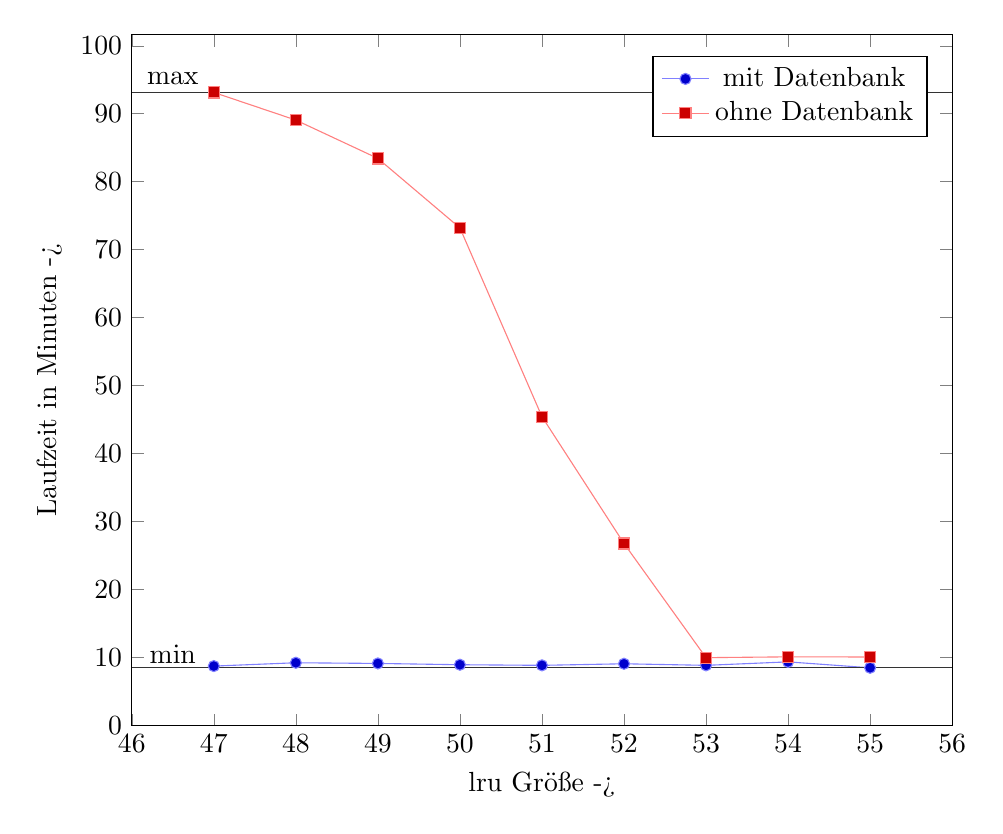
\begin{tikzpicture}
  \begin{axis}[
    width          = 12cm,
    %grid           = both, minor tick num=2,
    %title         = ??,
    xlabel         = \ac{lru} Größe ->,
    ylabel         = Laufzeit in Minuten ->,
    legend pos     = north east,
    ytick distance = 10,
    xmin=46, xmax=56,
    ]

    \tikzstyle{nodetext}=[draw=white, fill=white, draw opacity=0, fill opacity=0, text opacity=1]

    \addplot+[sharp plot, blue!50] coordinates
    {(55, 8.48) (54, 9.35) (53, 8.84) (52, 9.07)
     (51, 8.84) (50, 8.93) (49, 9.12) (48, 9.22) (47, 8.73)};
    \addplot+[sharp plot,  red!50] coordinates
    {(55, 10.07) (54, 10.09) (53, 9.97) (52, 26.77)
     (51, 45.43) (50, 73.20) (49, 83.43) (48, 89.07) (47, 93.14)};

     \addplot[sharp plot,  black!80] coordinates %min
     {(56, 8.48) (46, 8.48)};
     \addplot[sharp plot,  black!80] coordinates %max
     {(56, 93.14) (46, 93.14)};

     \node[nodetext] at (46.5, 10.48) {min};
     \node[nodetext] at (46.5, 95.14) {max};

    \legend{mit Datenbank, ohne Datenbank}
  \end{axis}
\end{tikzpicture}
\caption[Laufzeiten des Systems mit und ohne Datenbank als Cache]{Laufzeiten des Systems (5 Epochs, 53 Datensätze) mit und ohne Datenbank als Cache und variabler \ac{lru} Größe}\label{cap:analyze}
\end{center}
\end{figure}\label{fig:analyze}
